\chapter{Appendix about the axion peaks}

The idea is to give them all for completeness.
\mnote{Also, put the axion wind plots here!}



\section{EB anti-parallel}
\begin{figure}
  \centering
  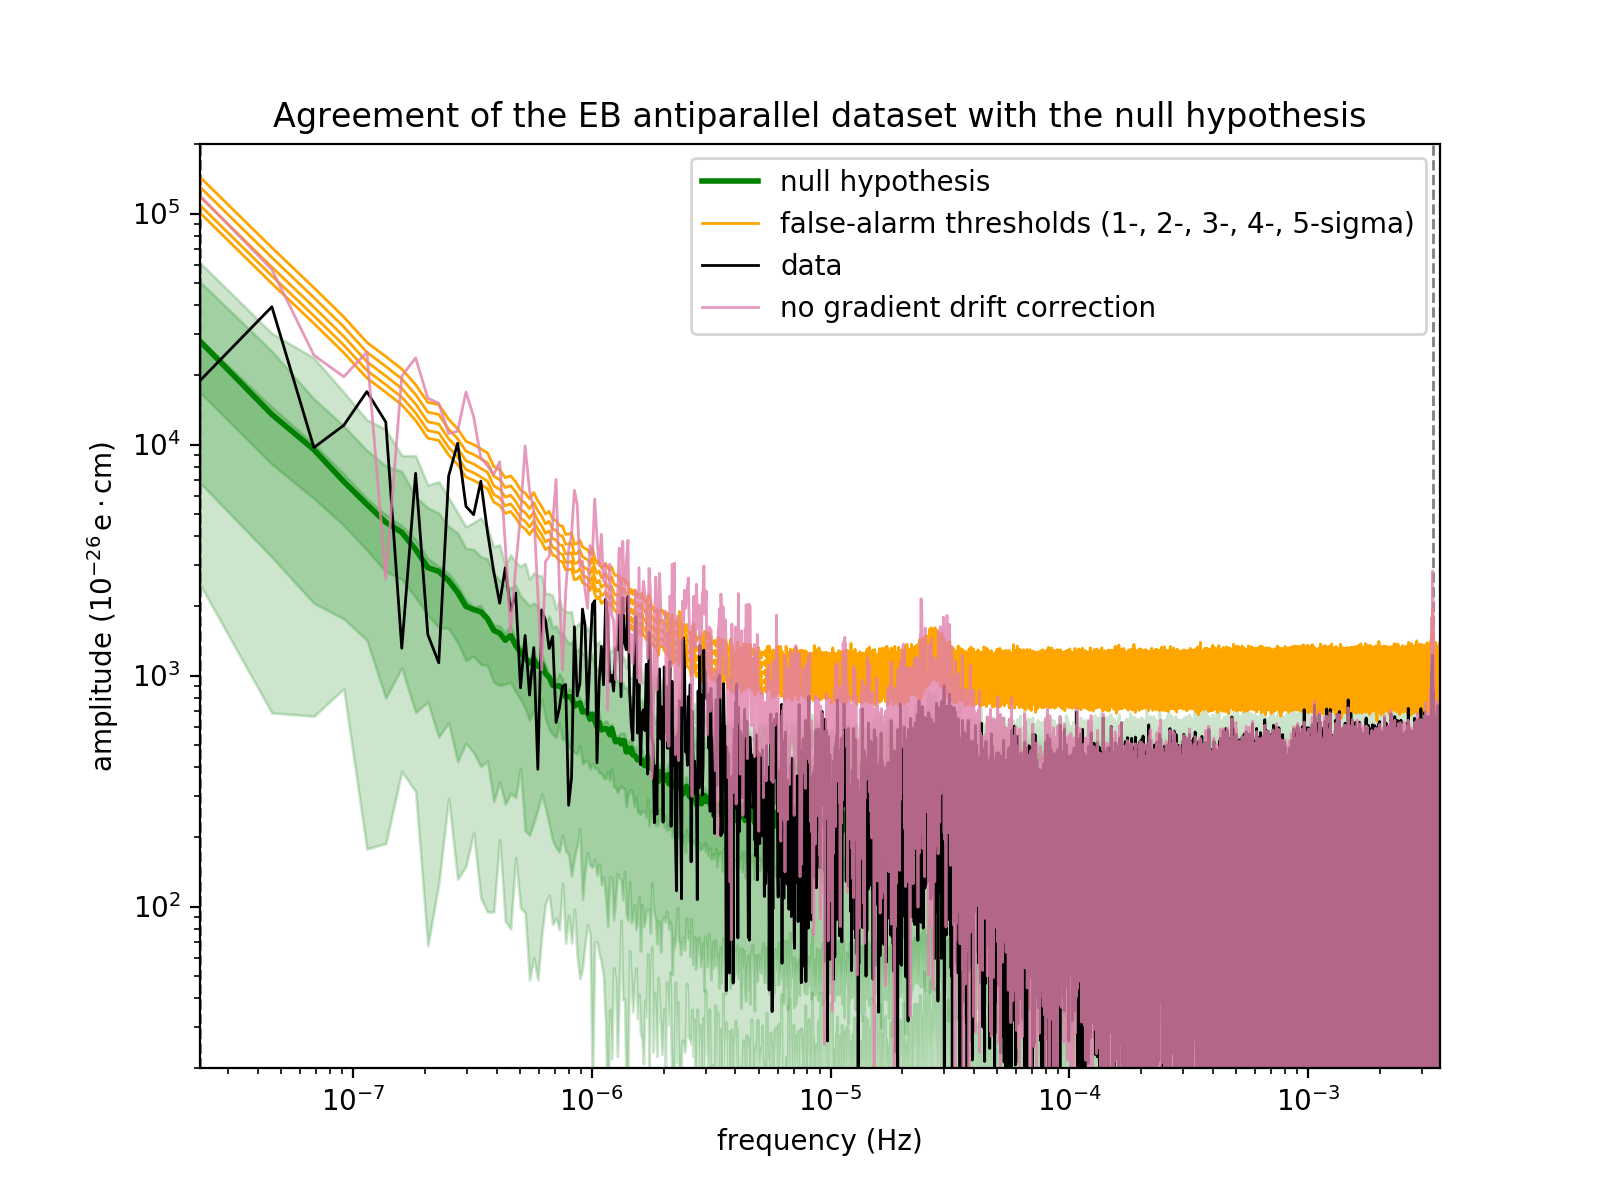
\includegraphics[width=\linewidth]{gfx/axions/AP_detection_and_no_GDC.png}
  \caption{\ldots}
  \label{fig:axions_AP_detection_and_no_GDC}
\end{figure}
\begin{figure}
  \centering
  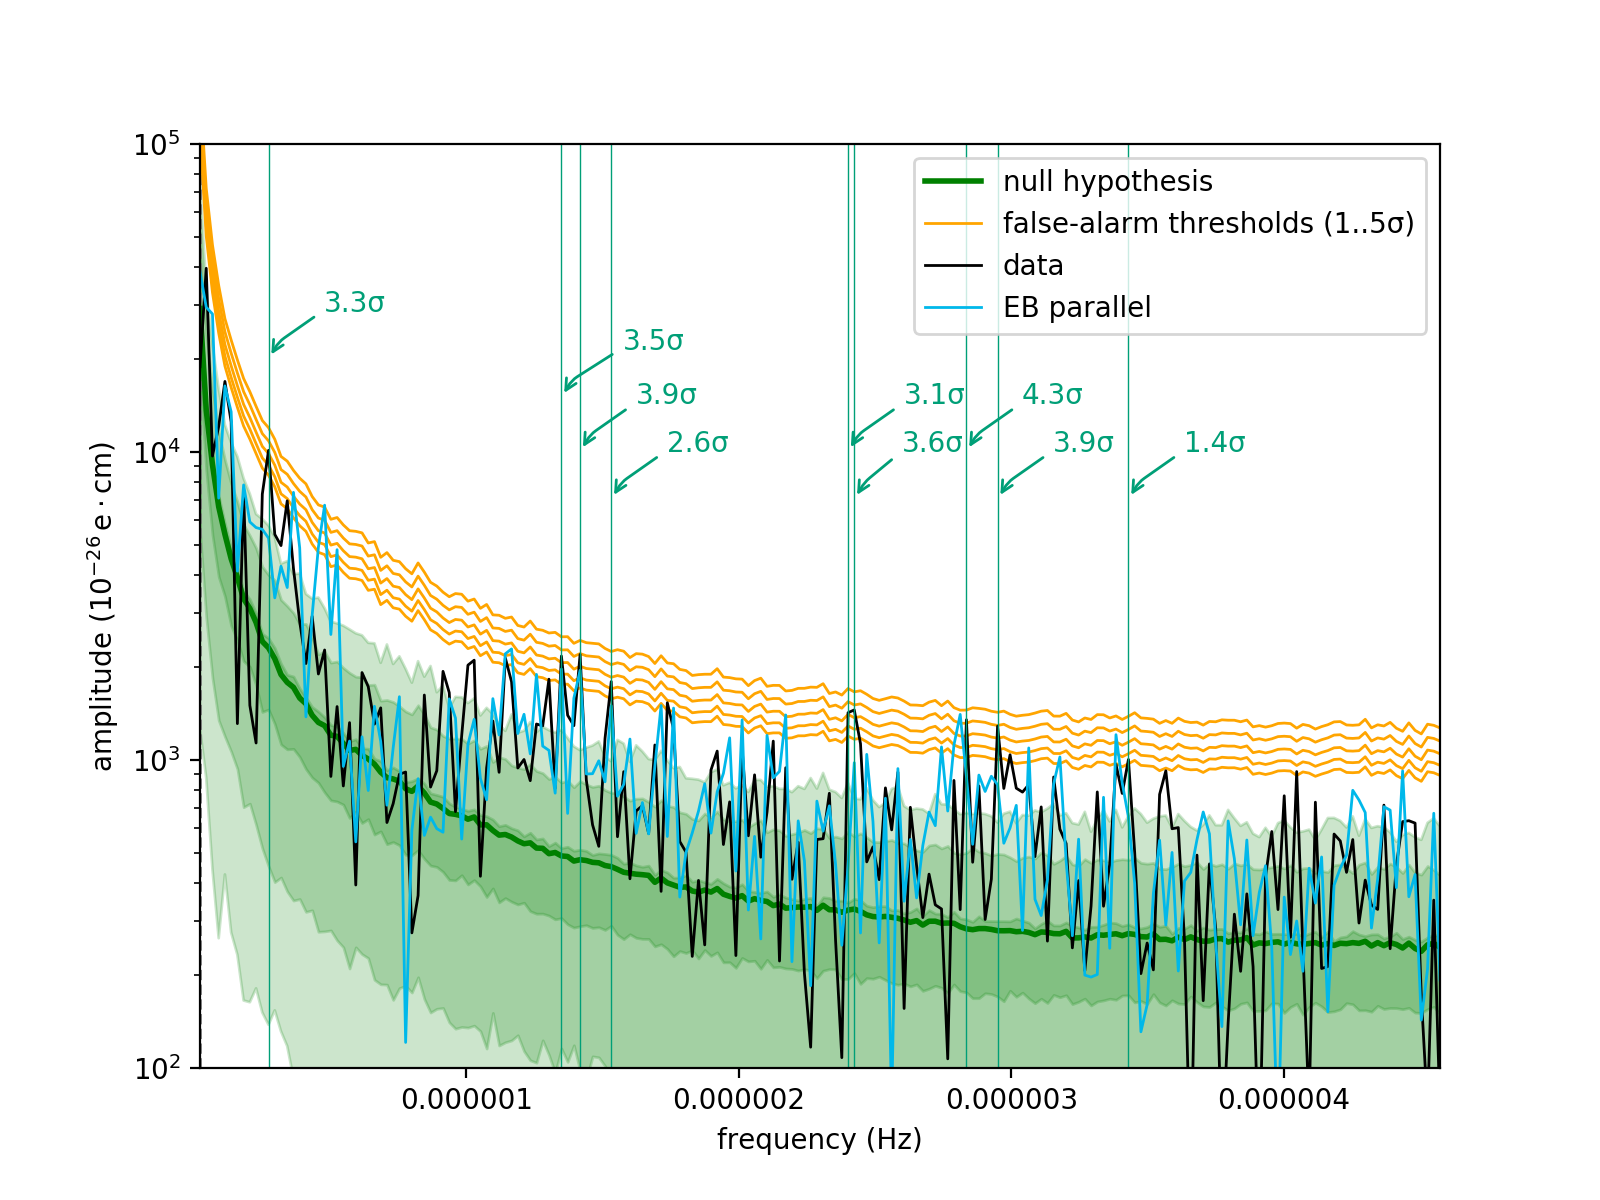
\includegraphics[width=\linewidth]{gfx/axions/AP_detection_area1.png}
  \caption{\ldots}
  \label{fig:axions_AP_detection_area1}
\end{figure}
\begin{figure}
  \centering
  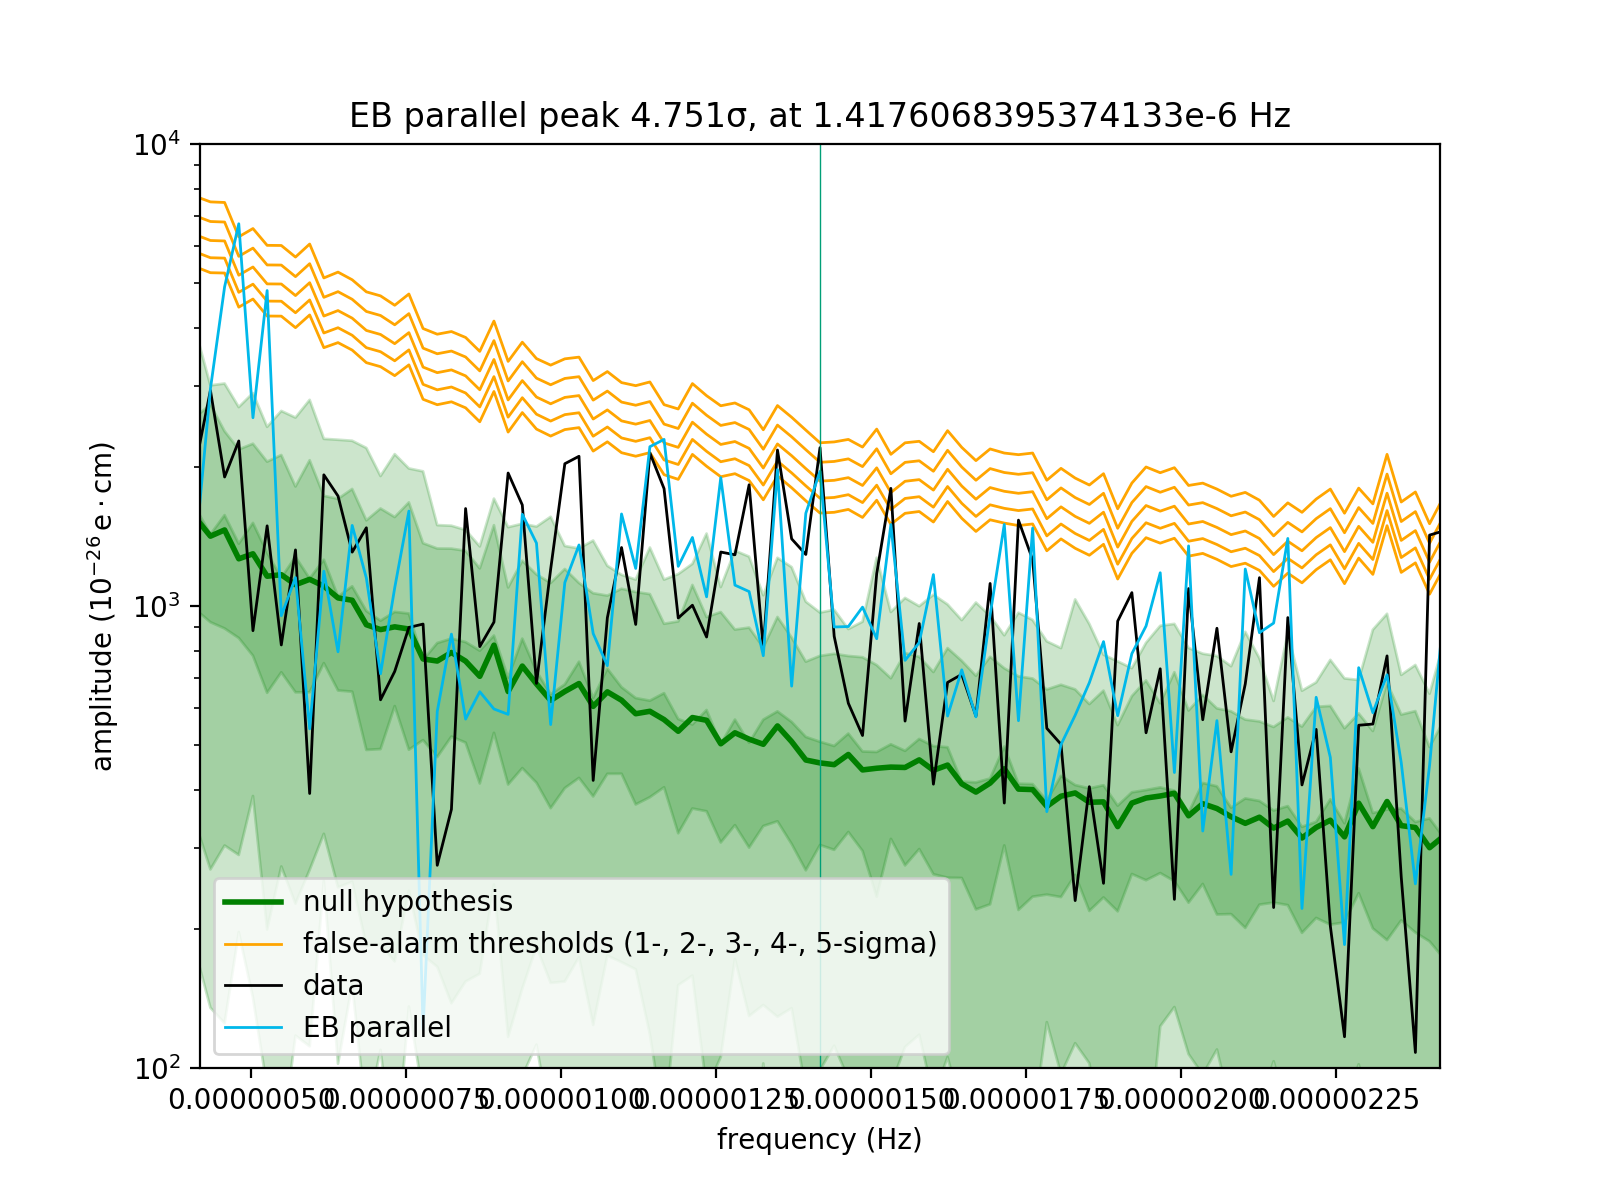
\includegraphics[width=\linewidth]{gfx/axions/AP_detection_peak_62.png}
  \caption{\ldots}
  \label{fig:AP_detection_peak_62}
\end{figure}
\begin{figure}
  \centering
  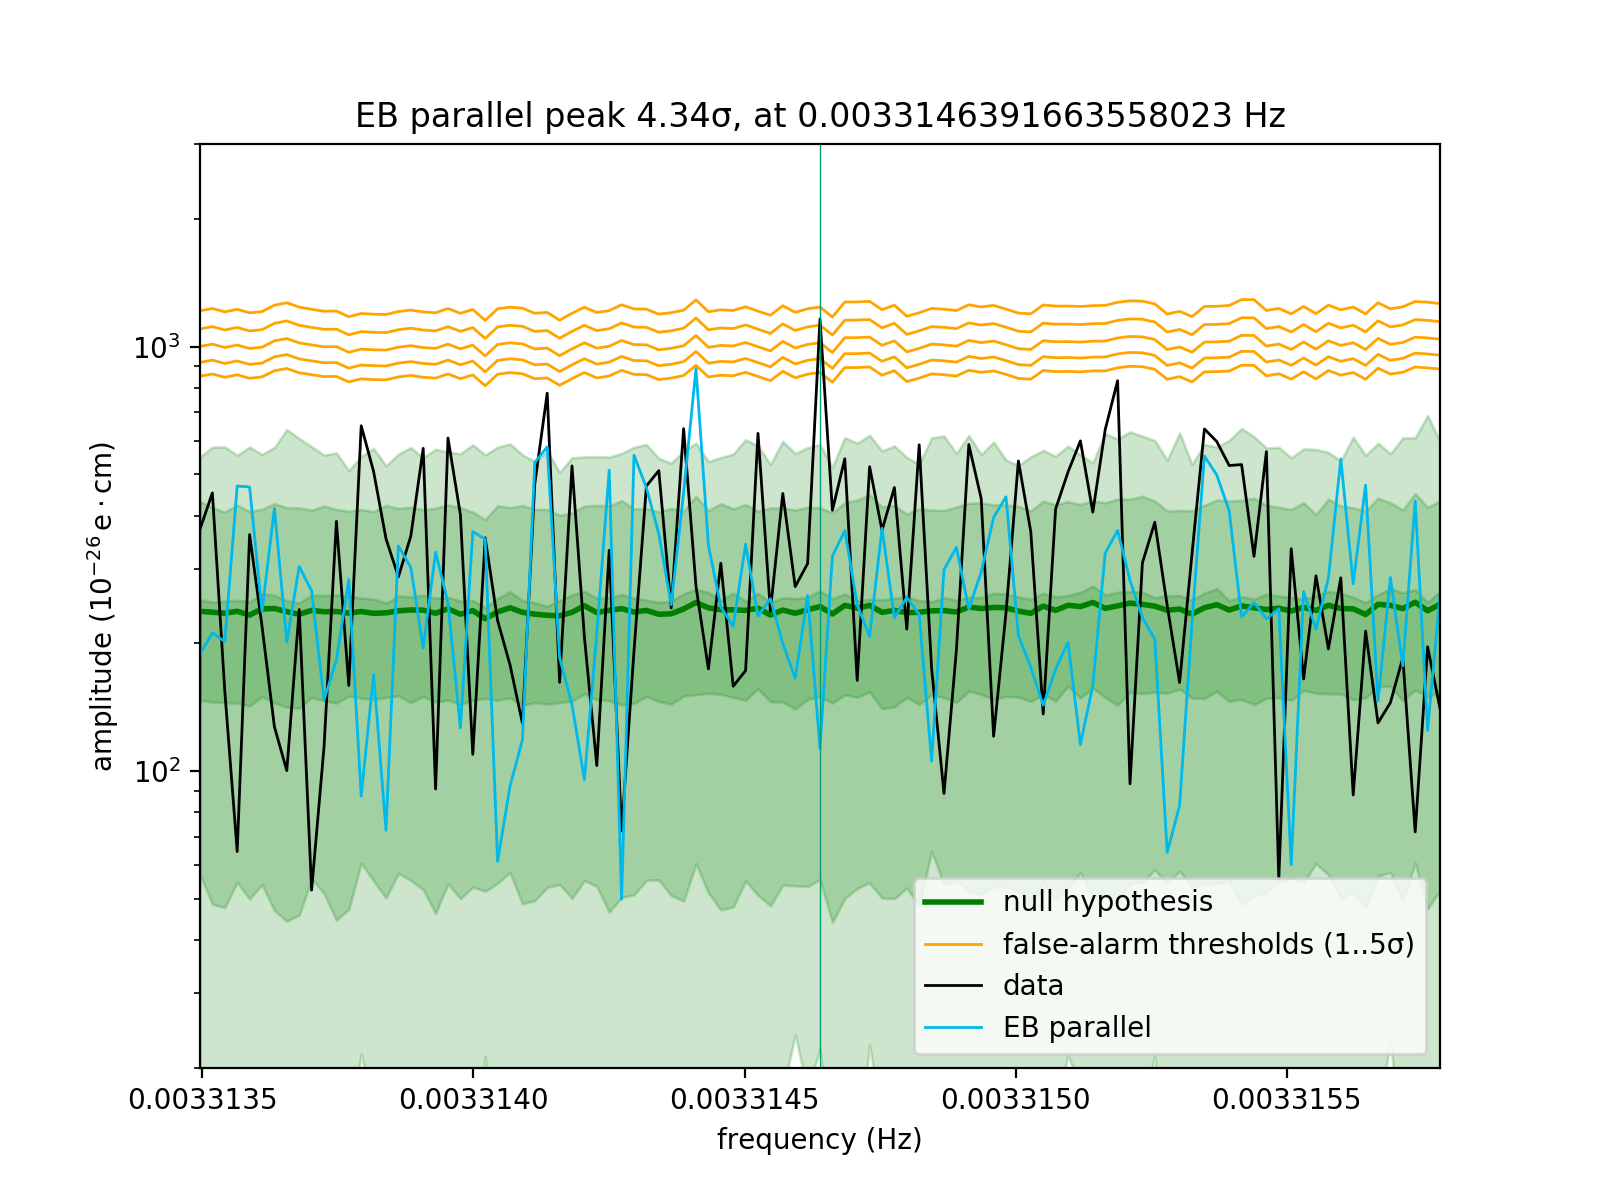
\includegraphics[width=\linewidth]{gfx/axions/AP_detection_peak_144968.png}
  \caption{\ldots}
  \label{fig:AP_detection_peak_144968}
\end{figure}


\section{EB parallel}

\begin{figure}
  \centering
  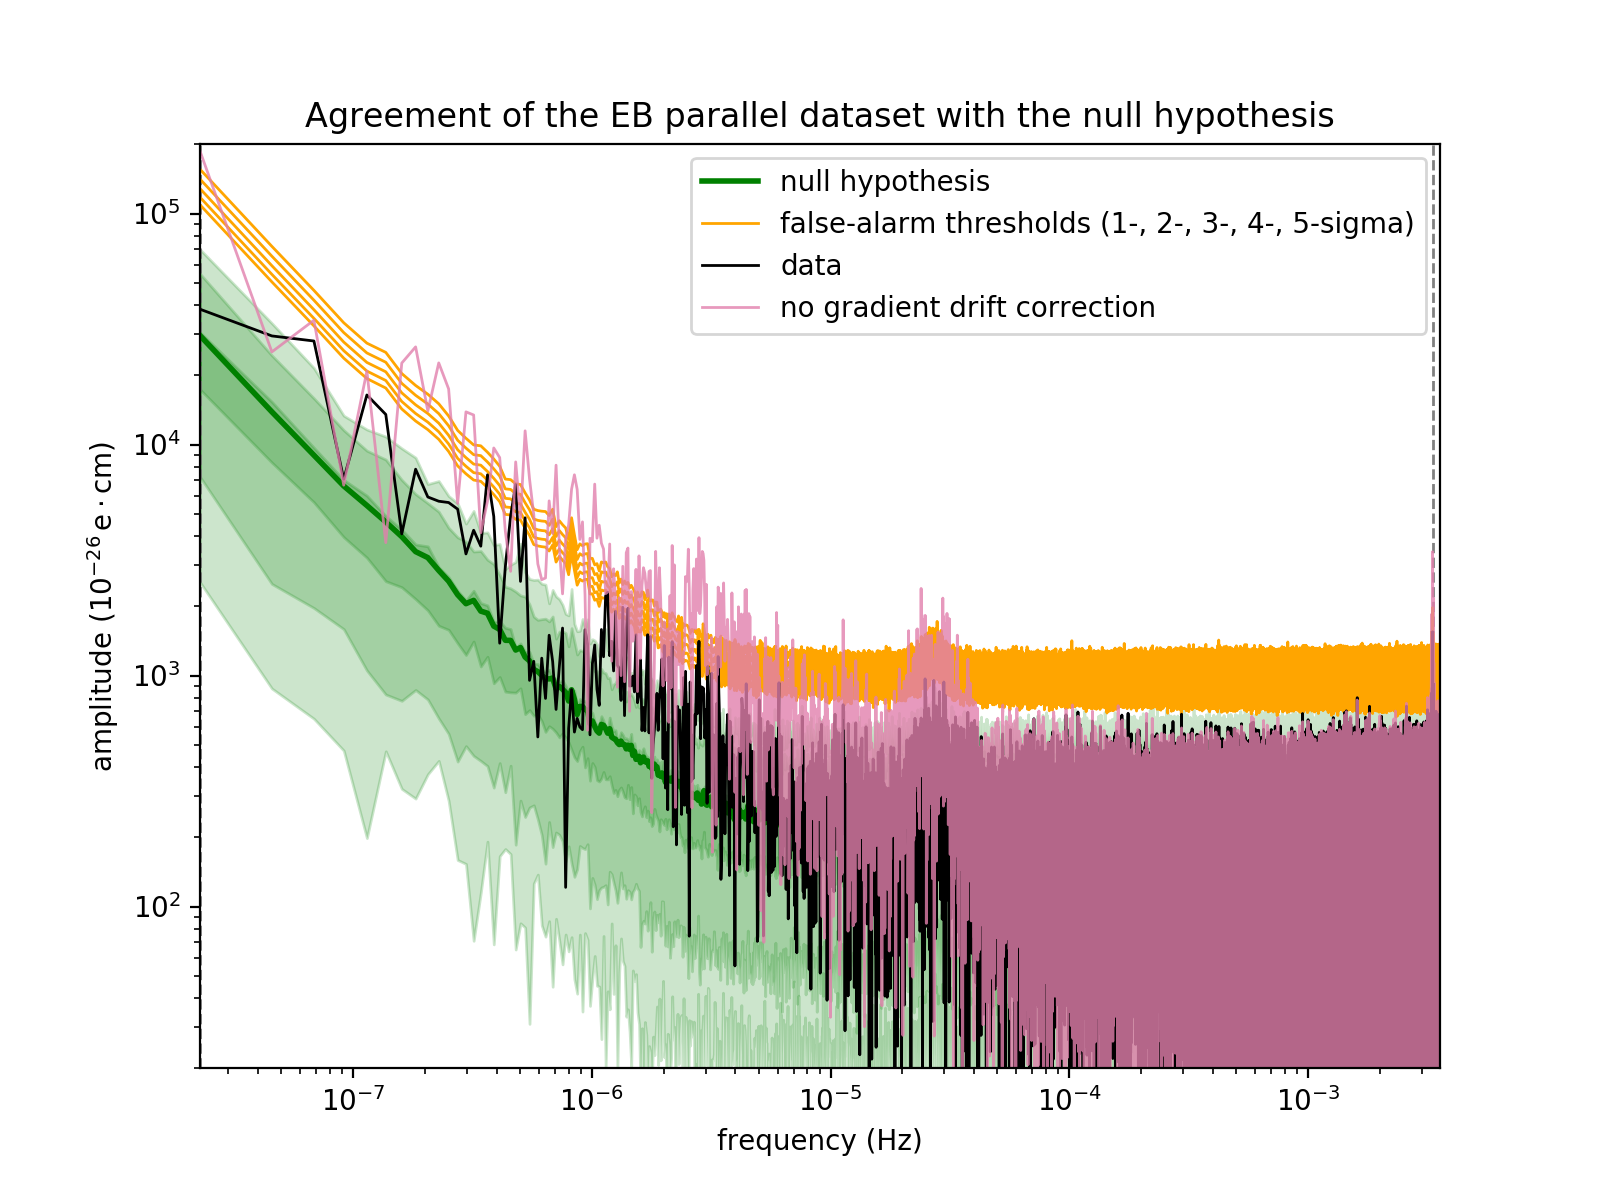
\includegraphics[width=\linewidth]{gfx/axions/P_detection_and_no_GDC.png}
  \caption{\ldots}
  \label{fig:P_detection_and_no_GDC}
\end{figure}
\begin{figure}
  \centering
  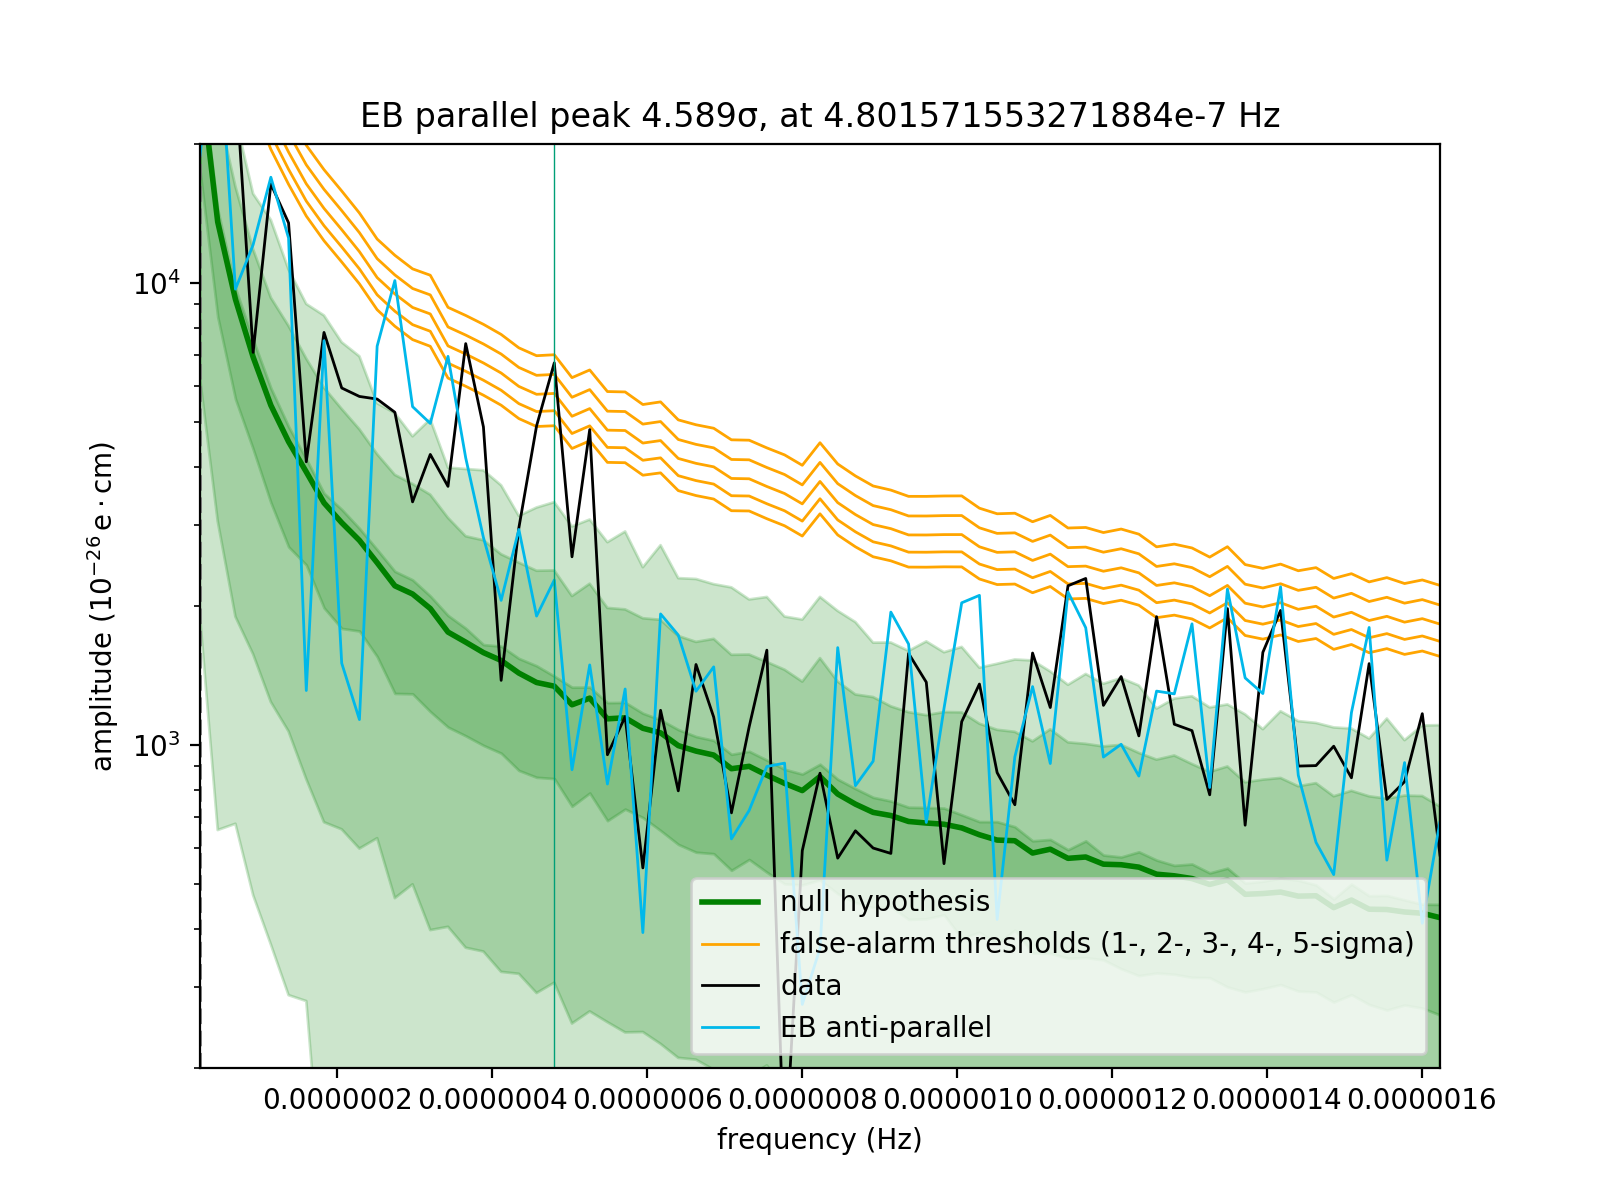
\includegraphics[width=\linewidth]{gfx/axions/P_detection_peak_21.png}
  \caption{\ldots}
  \label{fig:P_detection_peak_21}
\end{figure}
\begin{figure}
  \centering
  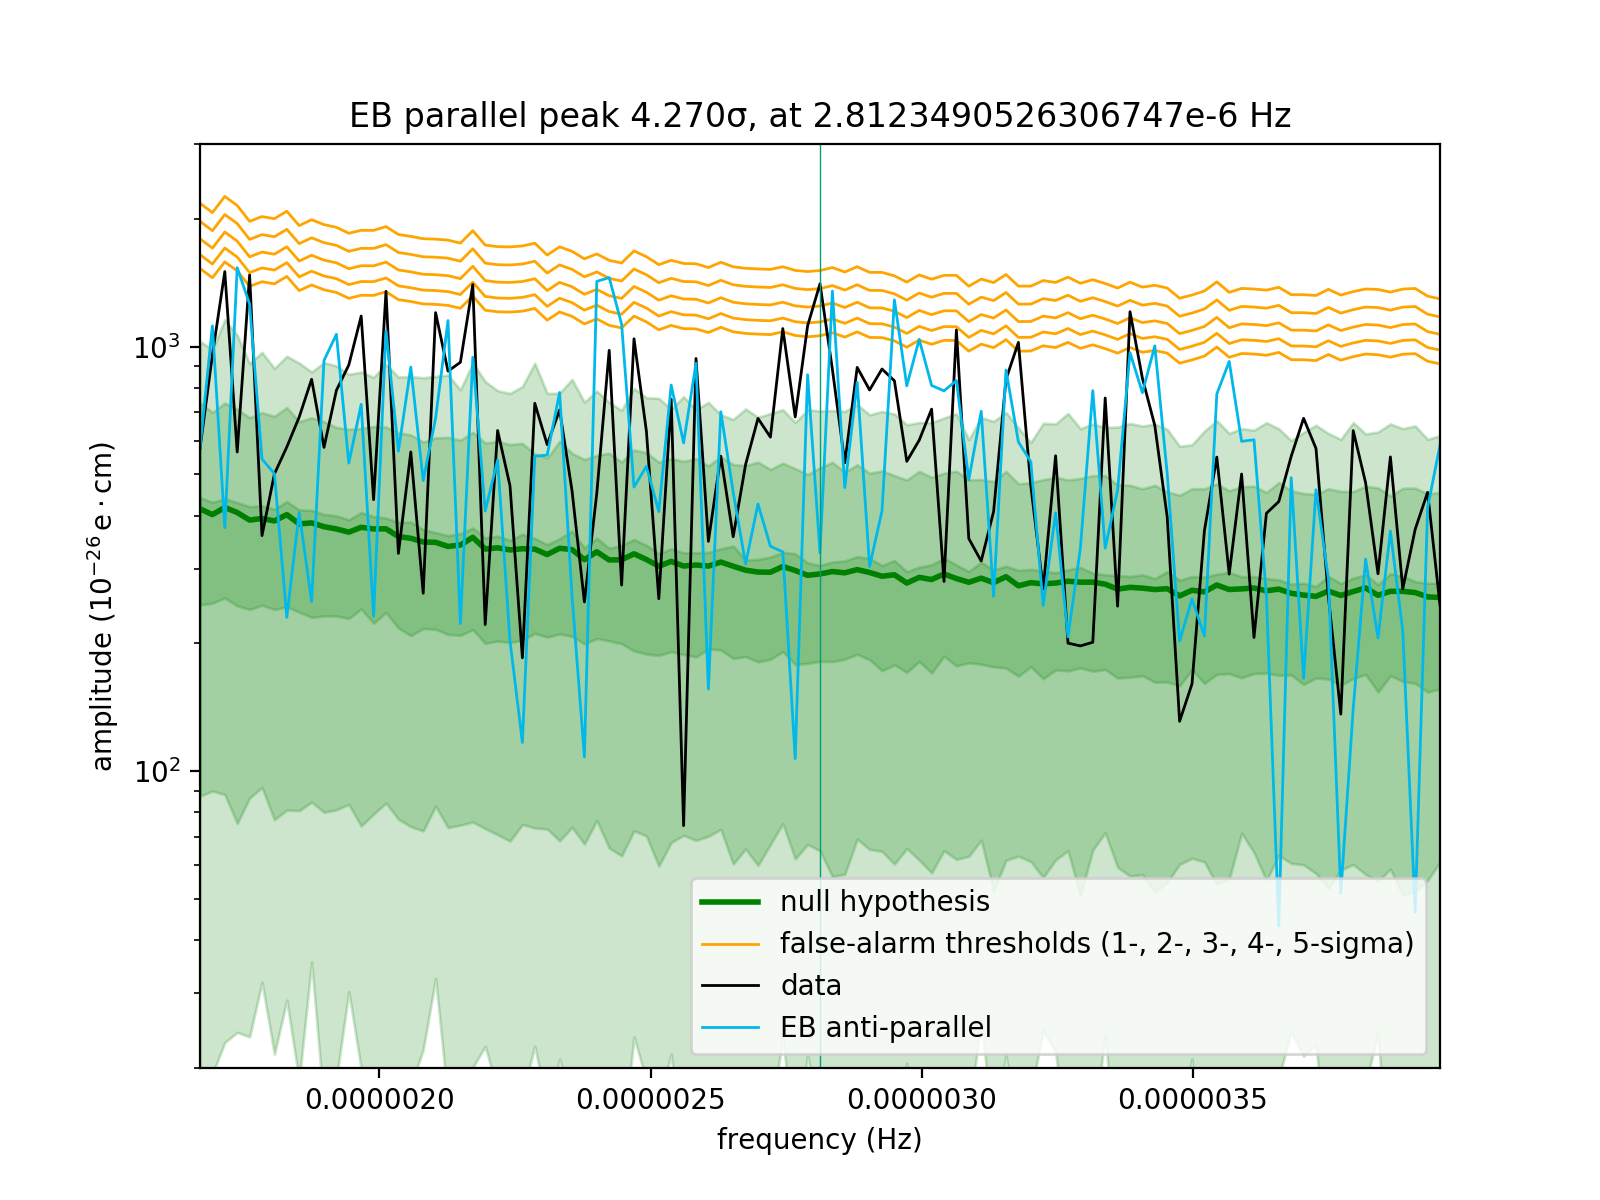
\includegraphics[width=\linewidth]{gfx/axions/P_detection_peak_123.png}
  \caption{\ldots}
  \label{fig:P_detection_peak_123}
\end{figure}
\begin{figure}
  \centering
  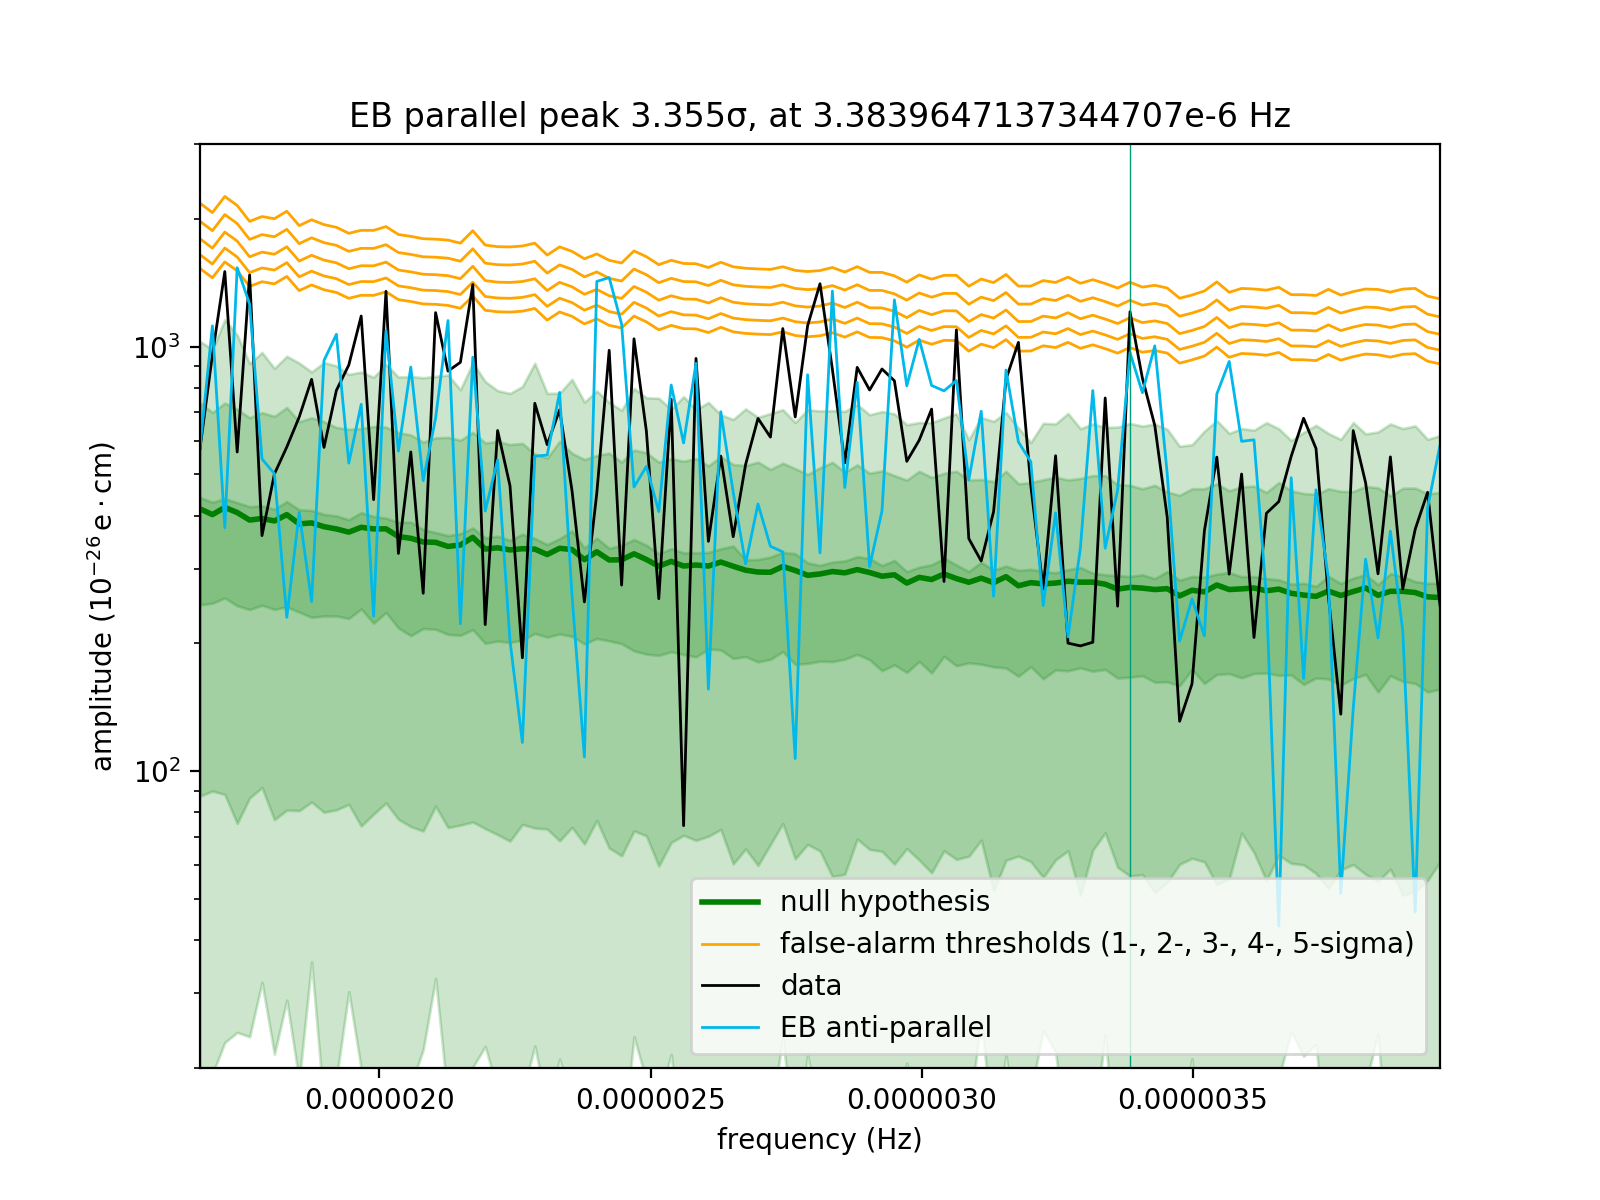
\includegraphics[width=\linewidth]{gfx/axions/P_detection_peak_148.png}
  \caption{\ldots}
  \label{fig:P_detection_peak_148}
\end{figure}
\begin{figure}
  \centering
  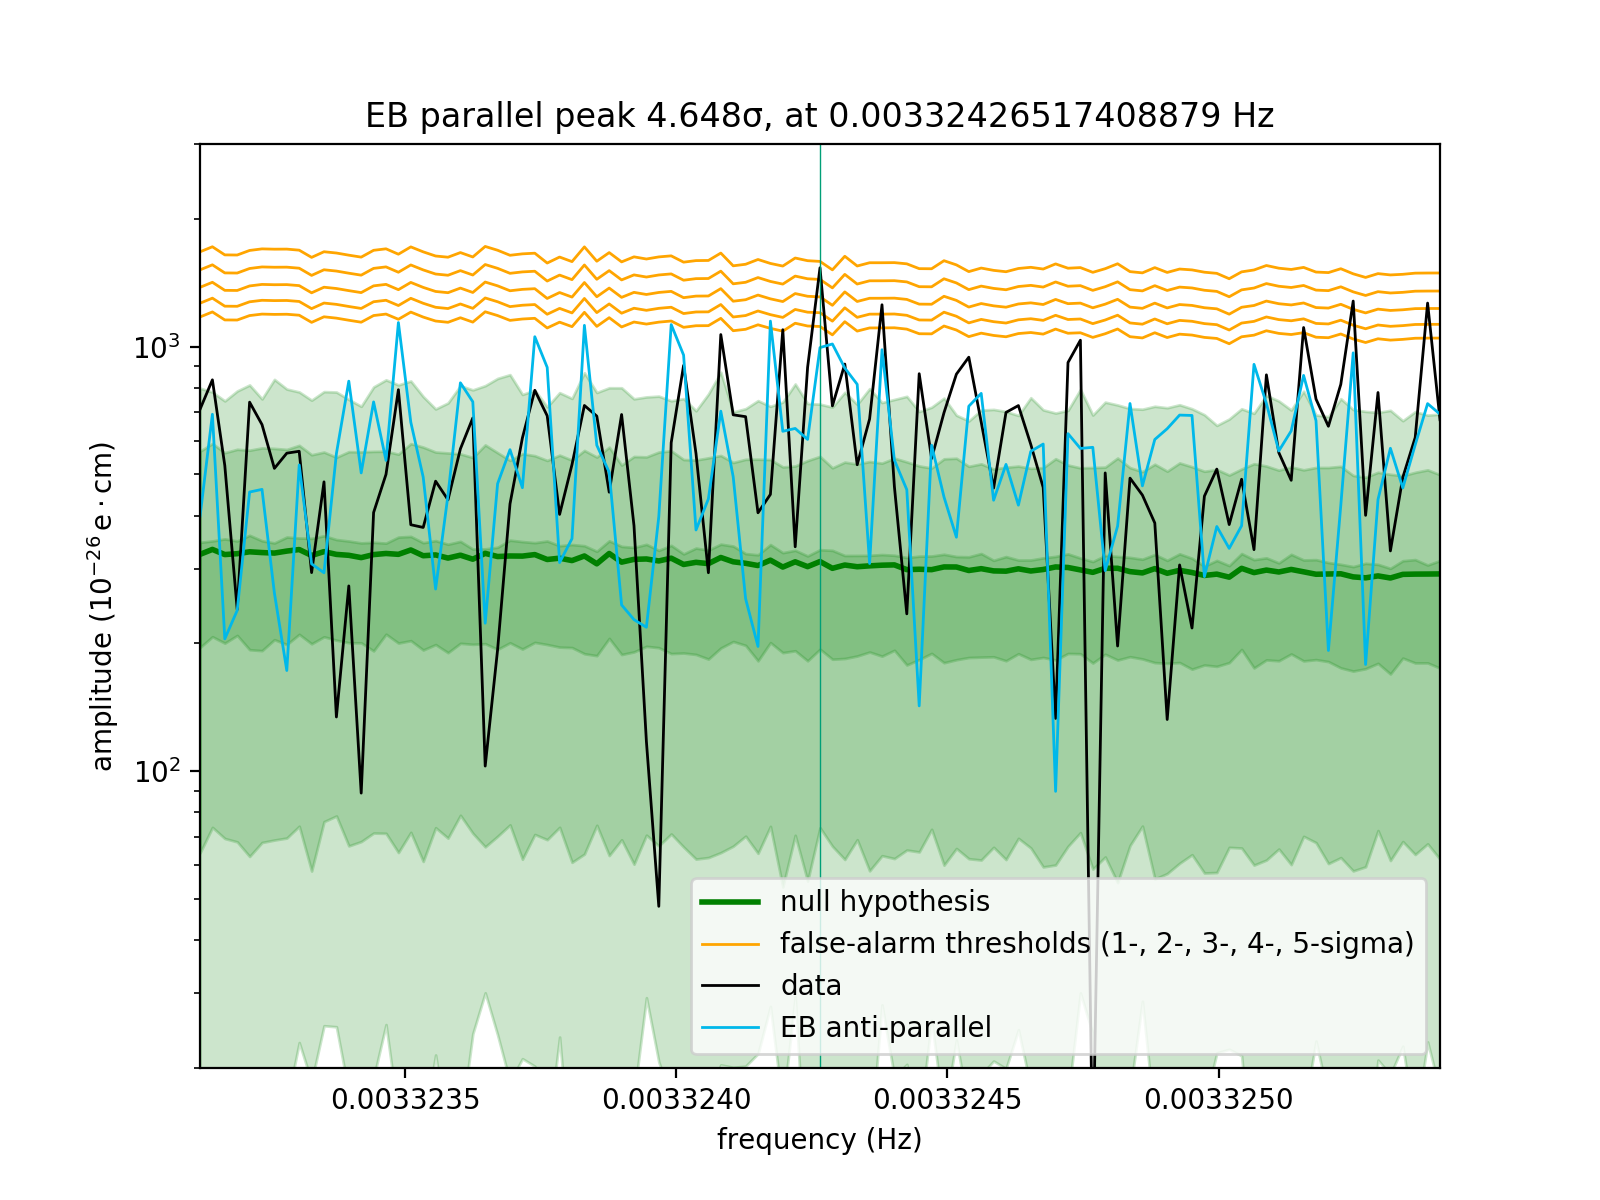
\includegraphics[width=\linewidth]{gfx/axions/P_detection_peak_145389.png}
  \caption{\ldots}
  \label{fig:P_detection_peak_145389}
\end{figure}
\begin{figure}
  \centering
  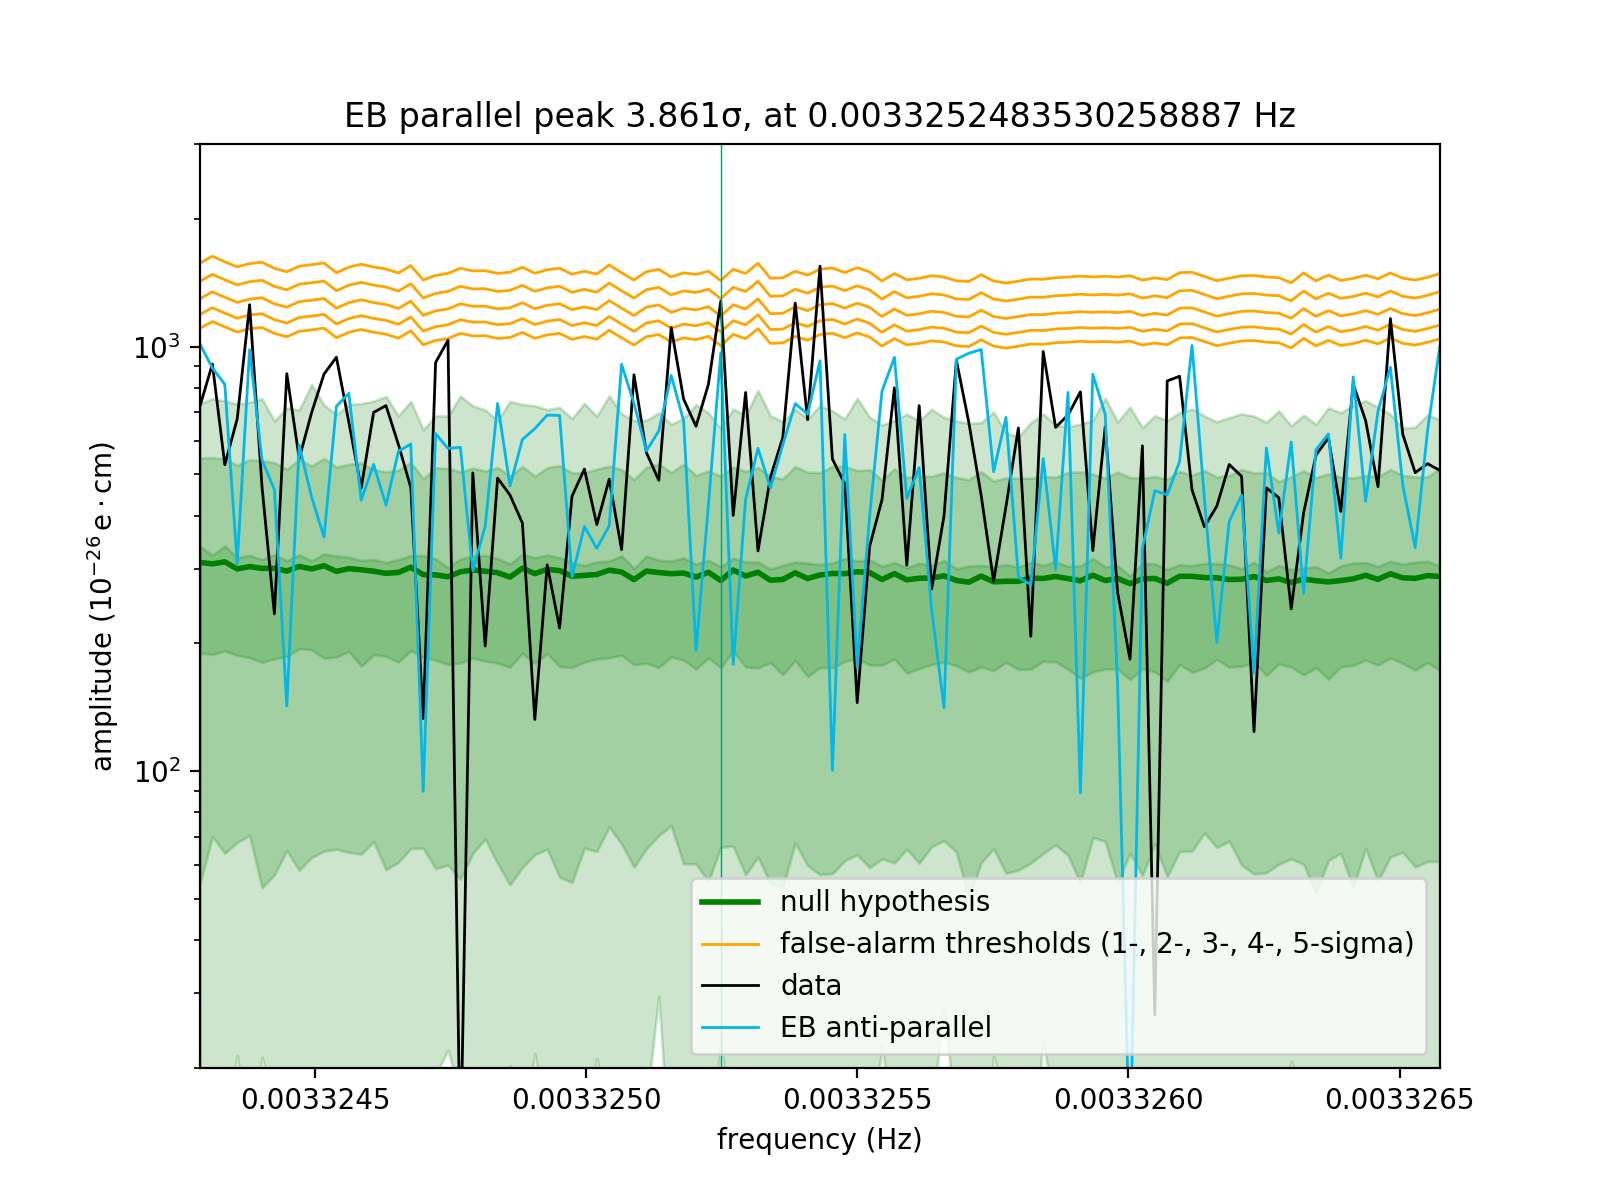
\includegraphics[width=\linewidth]{gfx/axions/P_detection_peak_145432.png}
  \caption{\ldots}
  \label{fig:P_detection_peak_145432}
\end{figure}
\begin{figure}
  \centering
  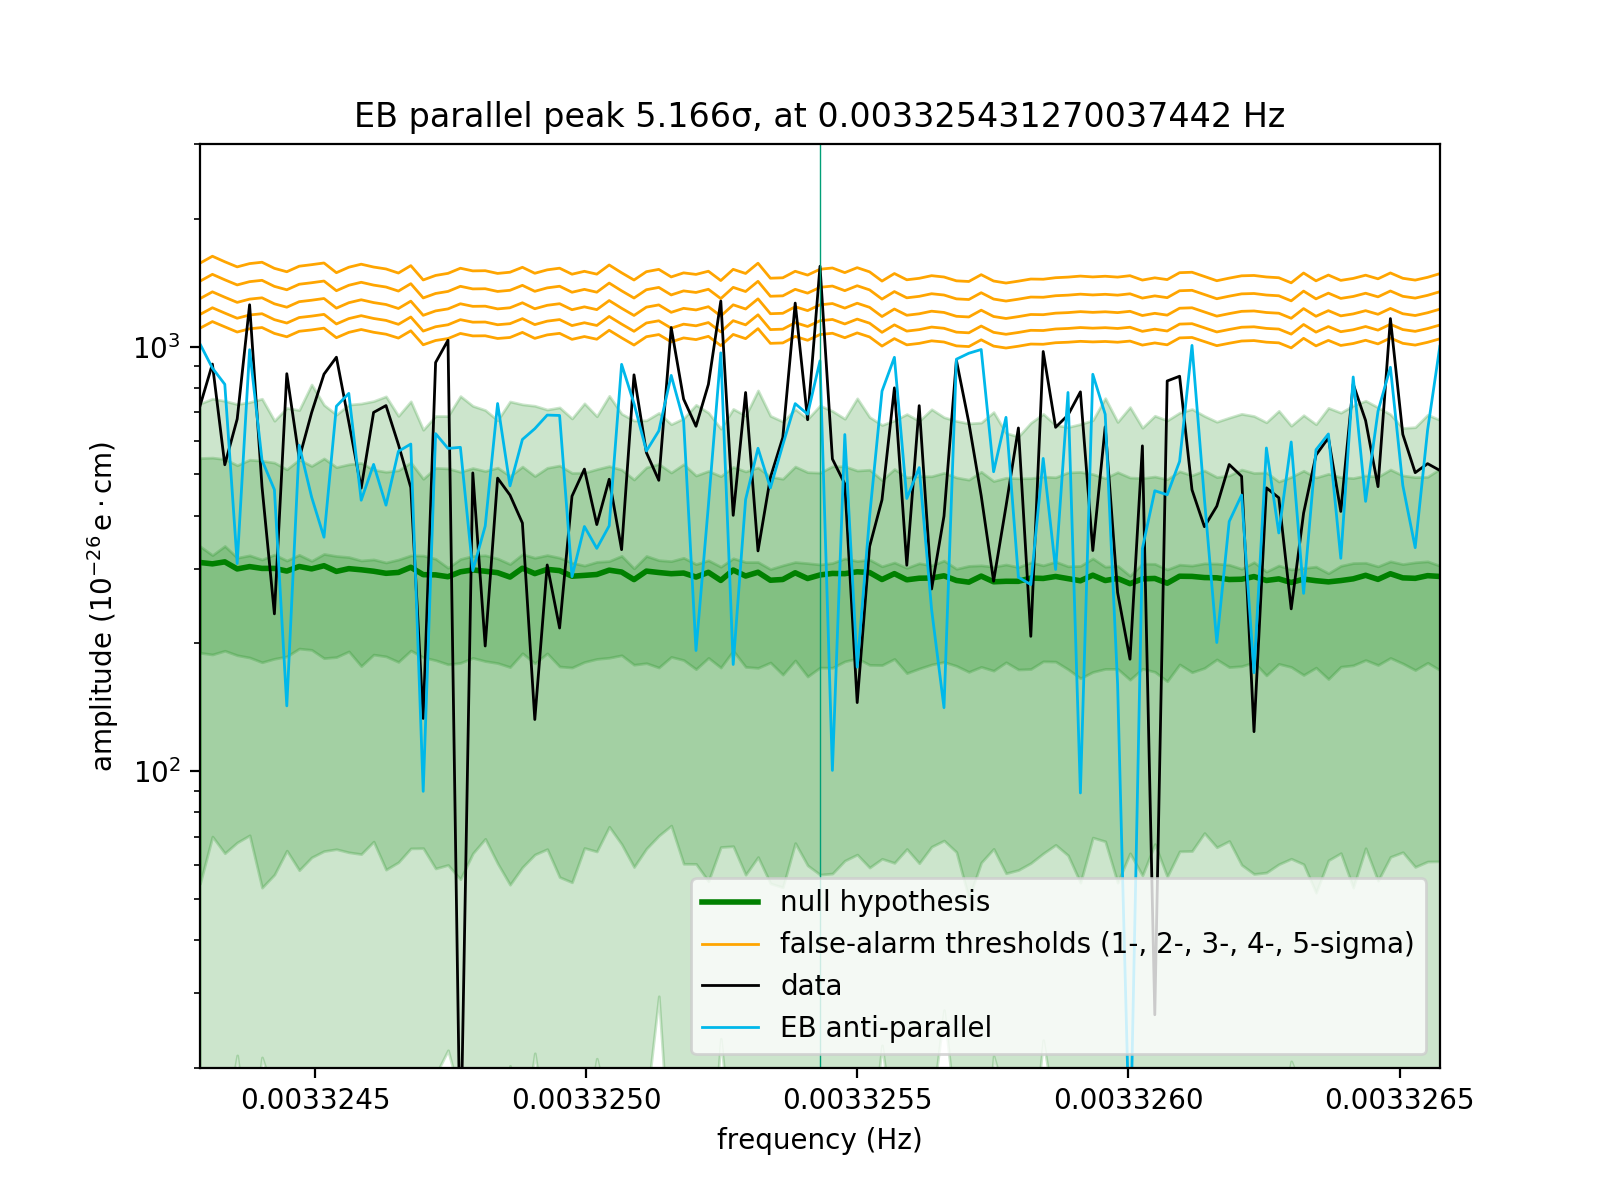
\includegraphics[width=\linewidth]{gfx/axions/P_detection_peak_145440.png}
  \caption{\ldots}
  \label{fig:P_detection_peak_145440}
\end{figure}


\section{E=0}

\begin{figure}
  \centering
  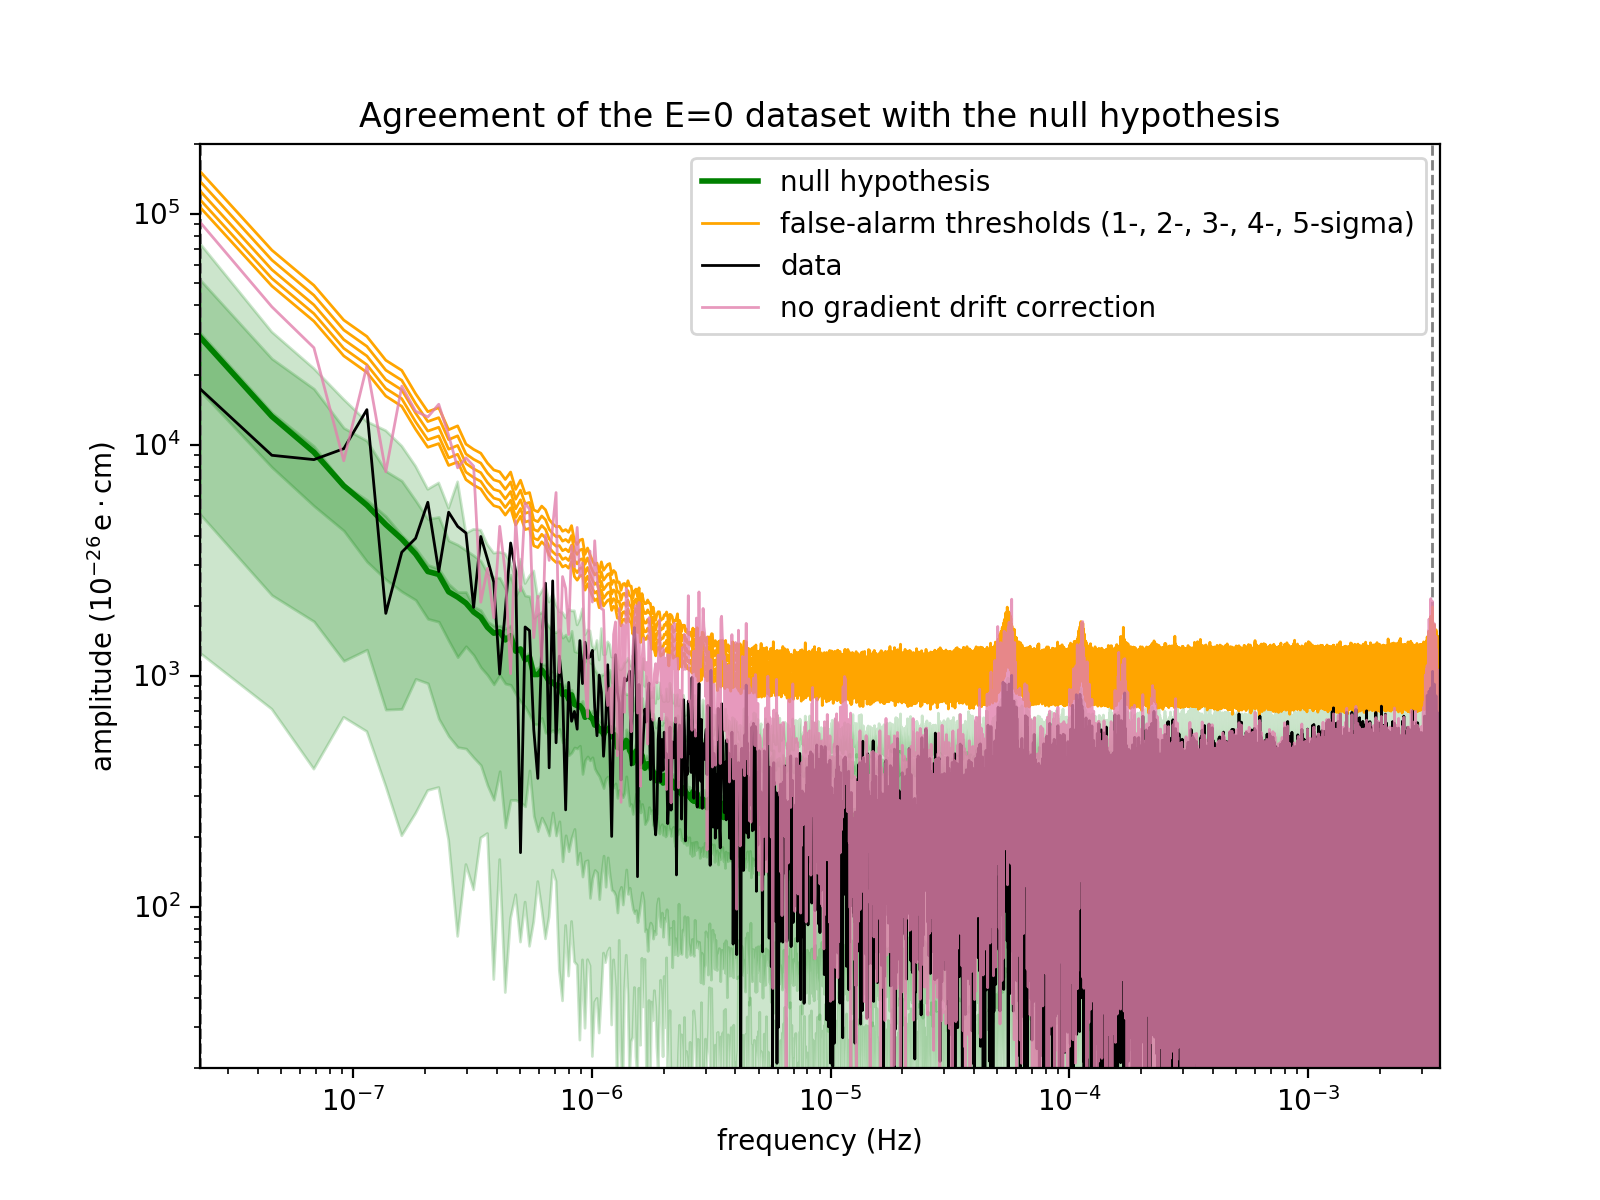
\includegraphics[width=\linewidth]{gfx/axions/E0_detection_and_no_GDC.png}
  \caption{\ldots}
  \label{fig:E0_detection_and_no_GDC}
\end{figure}
\begin{figure}
  \centering
  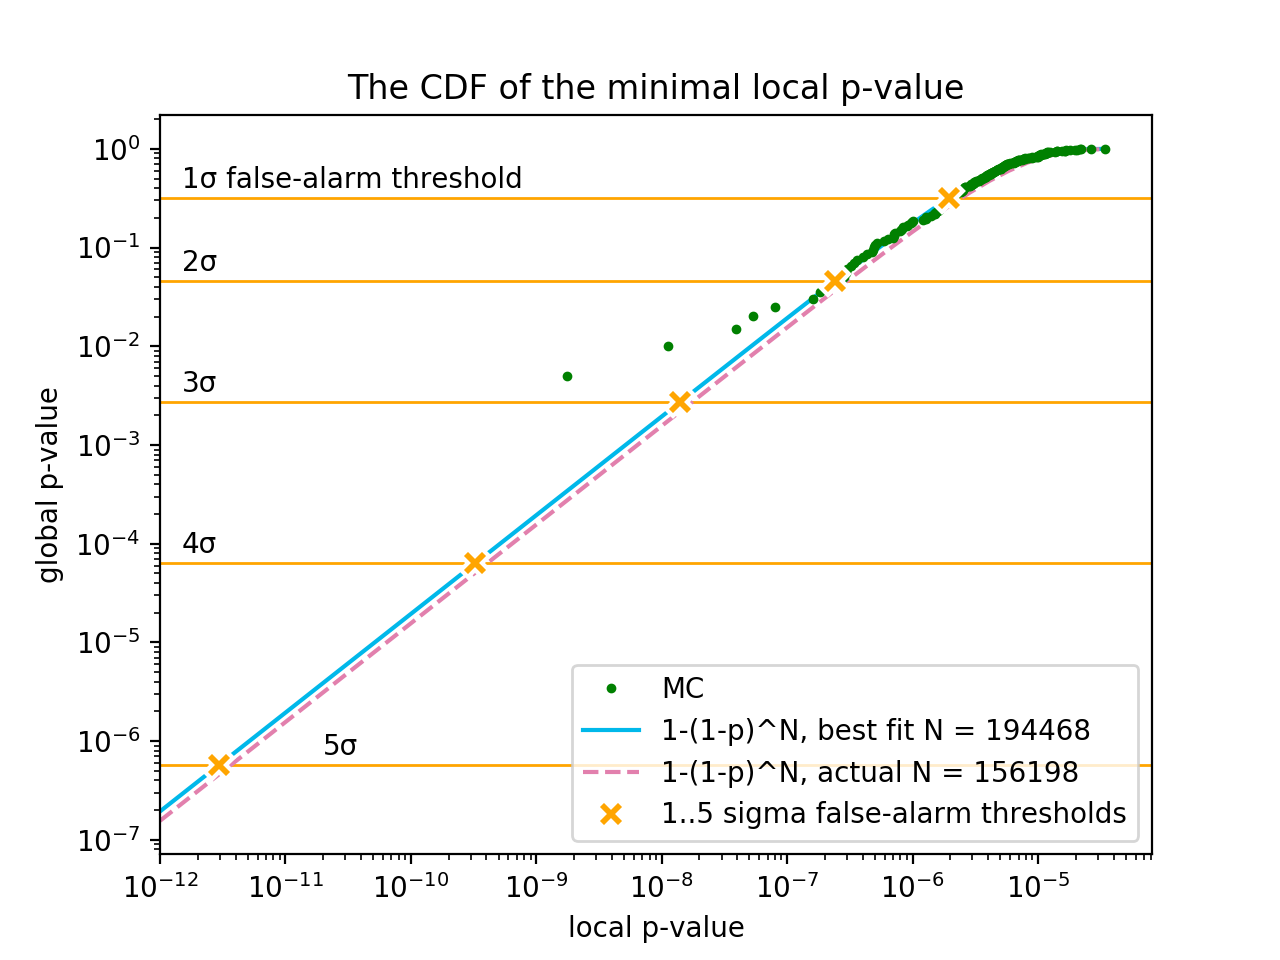
\includegraphics[width=\linewidth]{gfx/axions/E0_look-elsewhere.png}
  \caption{\ldots}
  \label{fig:E0_look-elsewhere}
\end{figure}
\begin{figure}
  \centering
  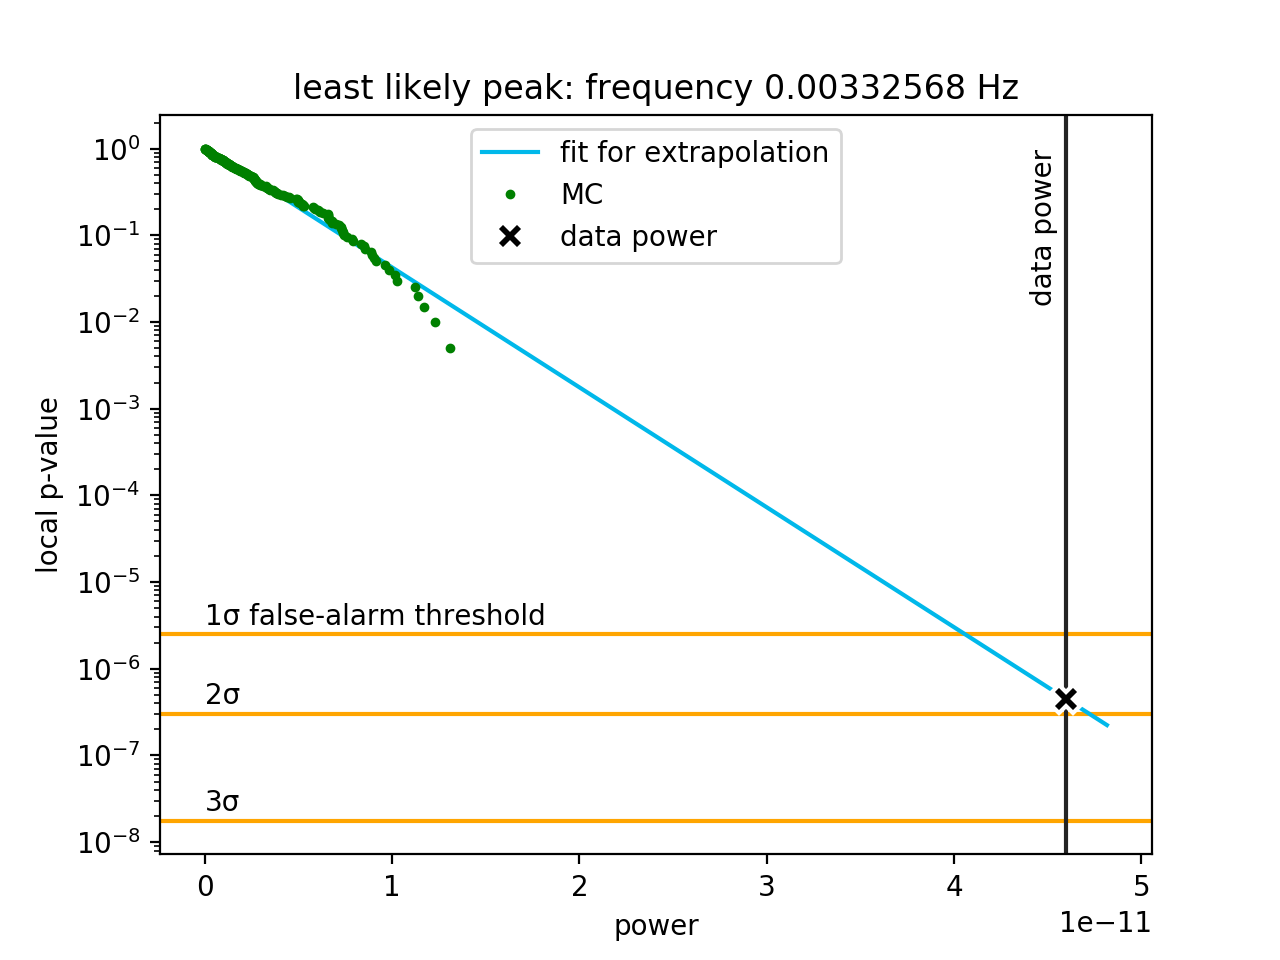
\includegraphics[width=\linewidth]{gfx/axions/E0_best_signal_candidate.png}
  \caption{\ldots}
  \label{fig:E0_best_signal_candidate}
\end{figure}
